\documentclass{standalone}
\usepackage{graphicx, standalone}
\usepackage[compat=1.1.0]{tikz-feynman}
\usepackage{tikz}
\usepackage{amsmath, amssymb}
\usepackage{euler}
\usepackage{fontspec}
\setmainfont{MinionPro}
\usepackage{comment}

\renewcommand{\k}{\ensuremath\text{k}}
\newcommand{\kp}{\ensuremath\text{k}'}
\newcommand{\q}{\ensuremath\text{q}}

\begin{document}

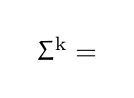
\begin{tikzpicture}[baseline=(current bounding box.center)]
	\node{$\Sigma^{\k}=$};
\end{tikzpicture}
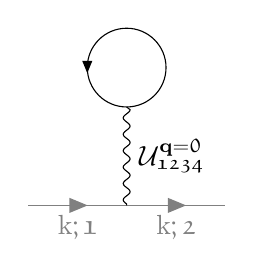
\begin{tikzpicture}[baseline=(current bounding box.base)]
	\begin{feynman}
		\vertex (a);
		\vertex[right=1.25cm of a] (b);
		\vertex[right=1.25cm of b] (c);
		\vertex[above=1.25cm of b] (b1);
		
		\vertex (u) at ($(b1)!0.5!(b)$);
		\node[right=0.1em of u] {$\mathcal{U}^{\textbf{q}=0}_{\mathfrak{1234}}$};
		
		\def\r{0.5}
		
		\path (b1)--++(90:\r) coordinate (A);
		\draw[fermion, arrow size=1pt] (A) circle(\r);		
		
		\diagram* {
			(a) -- [fermion, gray, edge label'=$\k;\mathfrak{1}$] (b) -- [fermion, gray, edge label'=$\k;\mathfrak{2}$] (c),
			(b) -- [photon] (b1)
		};	
	\end{feynman}
\end{tikzpicture}
\begin{tikzpicture}[baseline=(current bounding box.center)]
    \node {$-$};
\end{tikzpicture}
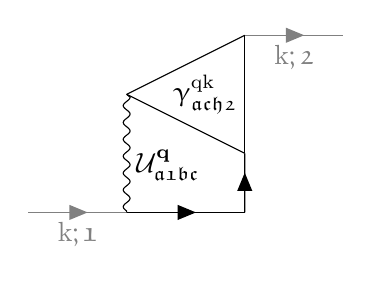
\begin{tikzpicture}[baseline=(current bounding box.base)]
	\begin{feynman}
		\vertex (a1);
		\vertex[right=1.25cm of a1] (a2);
		\vertex[right=of a2] (a3);
		\vertex[above=of a2] (b1);
		
		\vertex (i1) at ($(b1)+(1.5,-0.75)$);
		\vertex (i2) at ($(b1)+(1.5,+0.75)$);
		
		\node at ($(b1)+(1,0)$) {$\gamma_{\mathfrak{ach2}}^{\q\k}$};
		
		\vertex[right=1.25cm of i2] (b2);
		
		\diagram* {
			(a1) -- [fermion, gray, edge label'=$\k;\mathfrak{1}$] (a2),
			(a2) -- [photon, edge label'=$\mathcal{U}^{\textbf{q}}_{\mathfrak{a1bc}}$, pos=0.4] (b1),
			(b1) -- (i2) -- (i1) -- (b1),
			(a2) -- [fermion] (a3) -- [fermion] (i1),
			(i2) -- [fermion, gray, edge label'=$\k;\mathfrak{2}$] (b2),
		};
	\end{feynman}
\end{tikzpicture}
\begin{tikzpicture}[baseline=(current bounding box.center)]
    \node {$-$};
\end{tikzpicture}
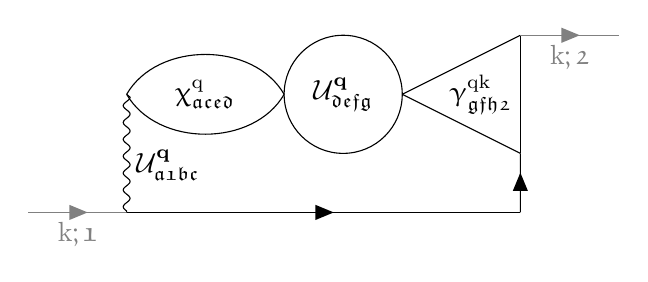
\begin{tikzpicture}[baseline=(current bounding box.base)]
	\begin{feynman}
		\vertex (a1);
		\vertex[right=1.25cm of a1] (a2);
		\vertex[right=2cm of a2] (a3);
		\vertex[right=of a3] (a4);
		\vertex[right=of a4] (a5);
		
		\vertex[above=of a2] (b1);
		\vertex[above=of a3] (b2);
		\vertex[above=of a4] (b3);		
		
		\vertex (i1) at ($(b3)+(1.5,-0.75)$);
		\vertex (i2) at ($(b3)+(1.5,+0.75)$);
		\node (u) at ($(b2)!0.5!(b3)$) {$\mathcal{U}^{\textbf{q}}_{\mathfrak{defg}}$};
		
		\node at ($(b3)+(1,0)$) {$\gamma_{\mathfrak{gfh2}}^{\q\k}$};
		
		\node at ($(b1)!0.5!(b2)$) {$\chi_{\mathfrak{aced}}^{\q}$};
		\draw (u) circle (0.75);
		
		\vertex[right=1.25cm of i2] (b4);
		
		\diagram* {
			(a1) -- [fermion, gray, edge label'=$\k;\mathfrak{1}$] (a2),
			(a2) -- [photon, edge label'=$\mathcal{U}^{\textbf{q}}_{\mathfrak{a1bc}}$, pos=0.4] (b1),
			(b1) -- [bend left=60] (b2) -- [bend left=60] (b1),
			(b3) -- (i2) -- (i1) -- (b3),
			(a2) -- [fermion] (a5) -- [fermion] (i1),
			(i2) -- [fermion, gray, edge label'=$\k;\mathfrak{2}$] (b4),
		};
	\end{feynman}
\end{tikzpicture}

\end{document}